\documentclass[12pt]{article}
\usepackage{polish}
\usepackage[utf8]{inputenc}
\usepackage{url}
\usepackage{hyperref}
\usepackage{multicol}
\usepackage{geometry}
\usepackage{fancyhdr}
\usepackage{graphicx}
\usepackage{enumitem}
\usepackage{mathtools, etoolbox}
\usepackage{blkarray}
\usepackage[showframe, nomarginpar]{geometry}


\setlist[itemize]{noitemsep, topsep=5pt}
\geometry{a4paper,total={170mm,257mm},left=20mm,top=20mm}
\setlist[itemize]{itemsep=7pt}
\setlist[enumerate]{itemsep=7pt}
\graphicspath{ {../} }

\pagestyle{fancy}
\rhead{Raport}
\lhead{}
\cfoot{}
\rfoot{Strona \thepage}
\fancypagestyle{firststyle}
{
\fancyhf{}
\fancyfoot[R]{Strona \thepage}
}

\newcounter{coun}[section]
\newenvironment{coun}[1][]{\refstepcounter{coun}\par\medskip
{\noindent\textbf{\thecoun #1. }}\leftskip=0em\rightskip=0em }{\par\medskip}


\newcommand\tabitem{\ifbool{firstrow}{\relax}{\\[\itemsep]}\boolfalse{firstrow}\makebox[\labelwidth][r]{\textbullet}\hspace*{\labelsep}}
\newbool{firstrow}
\newenvironment{braceditemize}[1][]{%
\booltrue{firstrow}
\vspace*{\topsep}\par\noindent
\setlength\BAextrarowheight{\parsep}\begin{blockarray}{@{}l <{\enspace}\Right{\}}{#1}}}
{\rule[-\itemsep-\parsep]{0pt}{\itemsep + \parsep}\end{blockarray}}


\begin{document}
\title{Raport \\  (środowisko agenta i reprezentacja wiedzy)}
\author{Marcin Woźniak \\ Filip Izydorczyk \\ Hubert Wrzesiński \\ Przemysław Fierek\\ \\ \textbf{Grupa 5} }
\maketitle
\thispagestyle{firststyle}
\vspace{30}
Repozytorium: \url{https://github.com/linux923344/autonomiczny_saper/}} \\
\vspace{30}

Spis klas użytych w projekcie:
\begin{enumerate}
	\item Board
	
		\begin{enumerate}[label=(\roman*)]
		\item Board - jako argumenty przyjmuje X i Y, które sa rozmiarem renderowanego okna. Klasa odpowiada za renderowanie mapy i zarzadzanie obiektami na niej.
    		\item Direction - enum, który daje nam informacje, w którym kierunku ma sie poruszać postać.
		\item DirectionCalculator - obliczanie następnego punktu na podstawie podanych wcześniej x i y.
		\item EquipmentGui - klasa odpwoiedzialna za grafikę Ekwipunku
		\item EquipmentGuiControl - klasa odpowiedzlana za zbieranie narzędzi i umieszczanie ich w ekwipunku.
		\item GameStarter - odpowiada za wystartowanie całego programu, po wybraniu odpowiednich opcji z menu.
		\item MapReader - argumentem przy jej tworzeniu jest plansza czyli obiekt typu Board, na której MapReader bedzie tworzy l obiekty które sa przechowywane w zewnetrznym pliku.
		\item Point - klasa punktu
		\item WalkingType - typ chodzenia (Za pomocą uczenia maszynowego, lub algorytmów chodzenia)
		\end{enumerate}
	
	\item MapObjects
    	
		\begin{enumerate}[label=(\roman*)]
		\item Bombs:
			\begin{braceditemize}[Obiekty odpowiedzialne za renderowanie oraz logikę bomby]
  				\tabitem BombRed
  				\tabitem BombBlue
  				\tabitem BombYellow
			\end{braceditemize}
		\item Saper - przechowuje informacje potrzebne do wyrenderowania Sapera, podnoszenie rzeczy do ekwipunku oraz jakie zadania musi wykonać.
		\item Stone - klasa, która jest odpowiedzialna za informacje potrzebne do wyrenderowania
kamienia.
    		\item Tool - klasa, która jest odpowiedzialna za informacje potrzebne do wyrenderowania na-
rzedzia.
    		\item Water - klasa, która jest odpowiedzialna za informacje potrzebne do wyrenderowania wody.
		\end{enumerate}

	\item MenuWindow
    		\begin{enumerate}[label=(\roman*)]
		\item MenuWindow - klasa odpowiedzialna za wygenerowanie menu, dzięki któremu możemy wybrać mapę, po której chcemy się poruszać, oraz typ algorytmu, za pomocą któ©ego chcemy przejść daną mapę.
		\item AlgorythmType - enum, z pomocą którego wybieramy algorytmy w MenuWindow.
		\end{enumerate}
	\item Path Finder
    		\begin{enumerate}[label=(\roman*)]
		\item BestFirstSearch
			\begin{itemize}
			\item Vertex - tworzy wierzchołki grafu
			\item GraphCreatorBestFS - tworzy graf BestFirstSearch
			\item GraphBFS - przejście po grafie BestFirstSearch
			\end{itemize}
		\item BreathFirstSearch
			\begin{itemize}
			\item Vertex - tworzy wierzchołki grafu
			\item GraphCreatorBFS - tworzy graf BFS
			\item GraphBFS - przejście po grafie BFS
			\end{itemize}
		\item DepthFirstSearch
			\begin{itemize}
			\item Vertex - tworzy wierzchołki grafu
			\item GraphCreator - tworzy graf DFS
			\item Graph - przejście po grafie DFS
			\end{itemize}
		\end{enumerate}
	\item PathFinder- wywołuje poszczególne algorytmy na planszy
	\item VowpalVabbit
		\begin{enumerate}[label=(\roman*)]
		\item DataCreator - klasa która tworzy dane uczące dla Vowpal Wabbit
		\item CellState - stan komórki
		\item VowpalPredicter - przewidywanie kolejnych kroków za pomocą Vowpala
		\end{enumerate}
\end{enumerate}
\newpage 

\noindent\textbf{27.03.2019 r.}
\setcounter{coun}{0}\\
\coun {Zaprojektowanie diagramu klas.}\\
\begin{center}
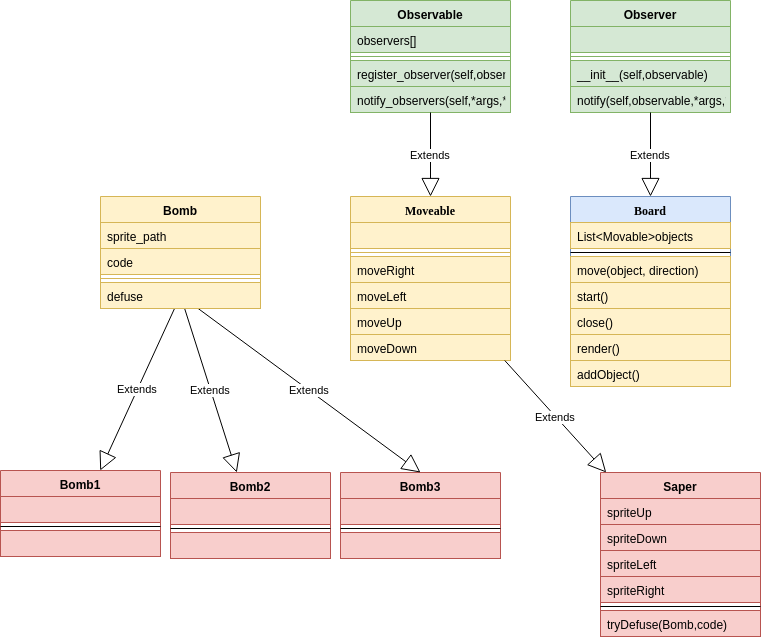
\includegraphics[scale=0.47]{logika.png}
\end{center}
\coun {Na podstawie diagramu, została stworzona klasa główna oraz jej podklasy.}
\coun {Został stworzony szablon planszy razem z umieszczonymi na niej bombami. }
\begin{center}
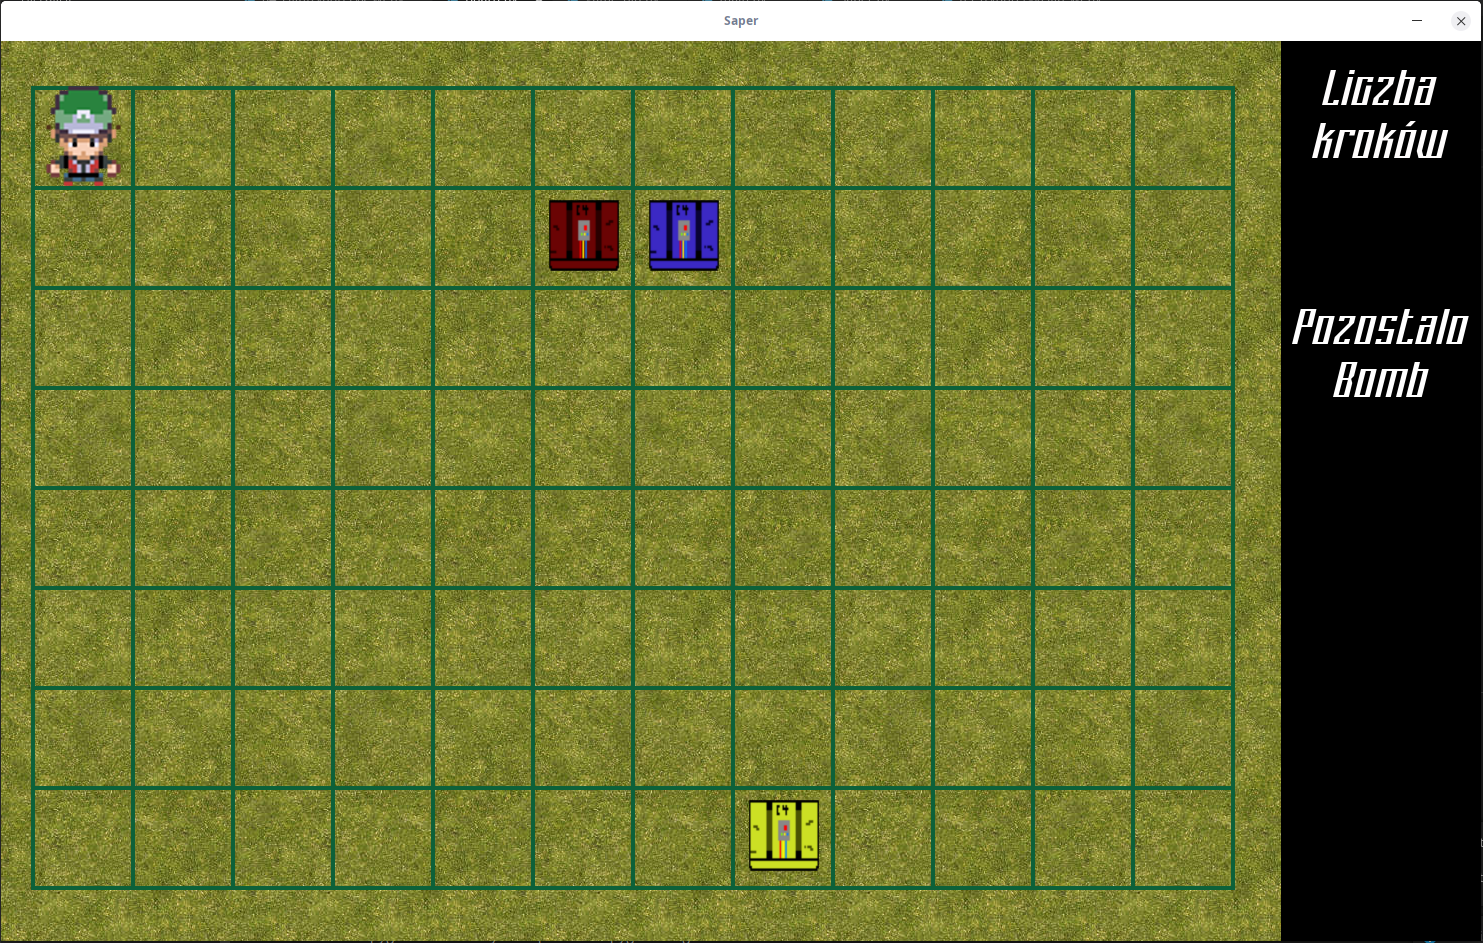
\includegraphics[scale=0.35]{plansza.png}
\end{center}
Na załączonym zrzucie ekranu widoczny jest saper czyli nasz Agent, oraz trzy kolorowe obiekty (bomby), które nasz agent ma za zadanie je rozbroić.\\

\noindent\textbf{10.04.2019 r.}\\
\setcounter{coun}{0}

W tym dniu została dokończona reprezentacja wiedzy w naszym projekcie.
Przedstawimy ją teraz:

\coun{Posiadamy trzy rodzaje bomb (czerwona, żółta, niebieska).}
\coun{Aby rozbroić bombę czewoną musimy posiadać narzędzie dodatkowo zmieścić się w wyznaczonym czasie. Jednostką czasu w naszym świecie jest jeden krok.}
\coun{Aby rozbroić pozostałe bomby Saper musi tylko do nich podejść, oczywiście jak nakrótszym czasie.}
\coun{Saper będzie wyznaczał drogę za pomocą algorytmu przeszukiwania grafu.}\\

\noindent\textbf{15.04.2019 r.}
\setcounter{coun}{0}\\

W tym dniu został zaimplementowany wyznaczanie ścieżki za pomocą algorytmu przeszukiwania DFS oraz kilka klas.\\

\noindent\textbf{17.04.2019 r.}
\setcounter{coun}{0}\\

Spisanie raportu i wypisanie wszystkich klas znajdujących się w projekcie.\\

\noindent\textbf{30.04.2019 r.}
\setcounter{coun}{0}\\

Dodanie ekwipunku i ustalenie zasad działania bomb. Bomby będą miały określony czas, a narzędzia będą potrzebne do rozbrojenia ich. \\

\noindent\textbf{6.05.2019 r.}
\setcounter{coun}{0}\\

Implementacja algorytmu BFS. \\ 

\noindent\textbf{14.05.2019 r.}
\setcounter{coun}{0}\\

Implementacja algorytmu Best-First Search. \\


\noindent\textbf{28.05.2019 r.}
\setcounter{coun}{0}\\

Dodanie klasy tworzącej dane uczące. Agent przechodzi graf, i z każdym krokiem zapisuje stan pól znajdujących się dookoła niego w kwadracie 7x7, do pliku.\\

\noindent\textbf{29.05.2019 r.}
\setcounter{coun}{0}\\

Ulepszenie algorytmu Best-First Search. Teraz nasz agent przechodzi graf zbierając po drodze wszystkie narzędzia znajdujące się na mapie\\

\noindent\textbf{01.06.2019 r.}
\setcounter{coun}{0}\\

Wykorzystanie zapisanych danych uczących przy Vowpal Wabbicie, a także dodanie licznika do bomb.\\

\noindent\textbf{02.06.2019 r.}
\setcounter{coun}{0}\\

Stworzenie większej ilości map do uczenia, a co za tym idzie, stworzenie większej ilości danych uczących.\\

\noindent\textbf{03.06.2019 r.}
\setcounter{coun}{0}\\

Agent jest nauczony, ale nie działa perfekcyjnie.\\

\noindent \textbf{Opis drzew decyzyjnych}\\

\noindent \textbf{Opis Volpal Wabbit}\\
\end{document}

